% !TEX TS-program = pdflatex
% !TeX program = pdflatex
% !TEX encoding = UTF-8
% !TEX spellcheck = en_US

\documentclass[xcolor=table]{beamer}


\def\accyear{2024-2025}

\institute{
	Laboratoire de la Communication dans les Systèmes Informatiques (LCSI)\\
	École  nationale Supérieure d'Informatique (ESI, ex. INI), Algiers, Algeria
}

\author[Abdelkrime Aries (\accyear)] %
{Abdelkrime Aries}

\titlegraphic{%
	\includegraphics[height=1cm]{../extra/logo/esi-logo.png}%
	\hspace*{2cm}%
	\includegraphics[height=1cm]{../extra/logo/lcsi-logo.png}%
	\hspace*{2cm}%
	
\includegraphics[height=1cm]{../extra/logo/esi.nlp.pdf}%
}%\hspace*{4.75cm}~

\date{Academic year: \accyear} %\today

\title[NLP]{Natural Language Processing} 

\usefolder{../extra/beamer}

\usetheme{Karimnlp} % Antibes Boadilla Warsaw

\beamertemplatenavigationsymbolsempty



\title[ESI - NLP: 02- ML for NLP]%
{Natural Language Processing\\Chapter 02\\Machine learning for NLP} 

\changegraphpath{../../img/ml4nlp/}

\begin{document}
	
%	\begin{frame}
%		\frametitle{Traitement automatique du langage naturel}
%		\framesubtitle{ML for NLP : Introduction}
%		
%		
%	\end{frame}
	
	\begin{frame}
		\frametitle{Natural Language Processing}
		\framesubtitle{ML for NLP: Algorithms}
		
		\begin{itemize}
			\item \optword{NB}: Naive Bayes
			\item \optword{LR}: Logistic regression
			\item \optword{SVM}: Support-Vector Machine
			\item \optword{NN}: Neural Network
			\item \optword{FFN}: Feed Forward Network
			\begin{itemize}
				\item \optword{MLP}: Multi-Layer Perceptron
				\item \optword{CNN}: Convolutional Neural Network
			\end{itemize}
			\item \optword{RNN}: Recurrent Neural Network
			\item \optword{HMM}: Hidden Markov Model
			\item \optword{MEMM}: Maximum-Entropy Markov Model
			\item \optword{CRF}: Conditional Random Field
		\end{itemize}
		
	\end{frame}
	
	\begin{frame}
		\frametitle{Natural Language Processing}
		\framesubtitle{ML for NLP: Types of models}
		
		\scriptsize
		\begin{tblr}{
				colspec = {p{.12\textwidth}lp{.37\textwidth}lp{.38\textwidth}},
				row{odd} = {lightblue},
				row{1} = {darkblue, fg=white, font=\bfseries, valign=m, halign=c},
				column{2,4}={white},
				column{1}={bg=darkblue, fg=white, font=\bfseries, valign=m},
				row{even} = {white},
				cell{1}{1}={white},
				colsep=3pt,
				rowsep=1pt,
			}
			
			&& Generative && Discriminative \\
			
			&&&&\\
			
			Text && NB && LR, SVM, MLP, RNN, CNN \\
			
			&&&&\\
			
			Sequence && HMM  && MEMM, CRF, RNN \\
			
		\end{tblr}
		
		\vfill
		
		\begin{itemize}
			\item \optword{Generative model}: a model that learns to generate features given a class:
			
			$\hat{Y} = \arg\max_k P(Y_k) P(X | Y_k)$
			
			\item \optword{Discriminative model}: a model that learns to estimate a class given some features: 
			
			$\hat{Y} = \arg\max_k P(Y_k | X)$
			
			
		\end{itemize}
		
	\end{frame}
	
	
	\begin{frame}
		\frametitle{Natural Language Processing}
		\framesubtitle{ML for NLP: Plan}
		
		\begin{multicols}{2}
			%	\small
			\tableofcontents
		\end{multicols}
	\end{frame}
	
	%===================================================================================
	\section{Machine learning}
	%===================================================================================
	
	\begin{frame}
		\frametitle{ML for NLP}
		\framesubtitle{\insertsection}
		
		\begin{itemize}
			\item This section is a review of ML algorithms
			\item Traditional ML algorithms: NB, LR, SVM
			\begin{itemize}
				\item Text features are engineered manually
			\end{itemize}
			\item MLP
			\begin{itemize}
				\item Text features can be learned/enhanced automatically
			\end{itemize}
			\item CNN
			\begin{itemize}
				\item Extracting relations between consecutive units
			\end{itemize}
			\item RNN
			\begin{itemize}
				\item Temporal dependent units processing
			\end{itemize}
		\end{itemize}
		
	\end{frame}
	
	\subsection{Traditional ML}
	
	\begin{frame}
		\frametitle{ML for NLP: \insertsection}
		\framesubtitle{\insertsubsection: Naive Bayes}
		
		Estimation 
		\[\hat{Y} = \arg\max_{Y_k} \log P(Y_k) + \sum_{j=1}^{N} \log P(X_j|Y_k)\]
		
		Training
		\[P(Y_k) = \frac{|\{y / y \in Y \wedge y = k\}|}{M}\]
		
		\begin{itemize}
			\item $|\{y / y \in Y \wedge y = k\}|$ is the number of samples belonging to class $k$ in the training dataset.
			\item $M$ is the number of samples in the training dataset.
			\item $P(X_j|Y_k)$ is calculated following one of three distributions: multinomial, normal or Bernoulli.
		\end{itemize}
		
	\end{frame}
	
	\begin{frame}
		\frametitle{ML for NLP: \insertsection}
		\framesubtitle{\insertsubsection: Logistic Regression}
		
		Estimation 
		\[\hat{Y} = \arg\max_{k} Softmax(\sum_{j=1}^{N} \theta_j X_j + \theta_0)\]
		
		Training
		\[J_\theta = \frac{-1}{M} \sum\limits_{i=1}^{M} \sum_{k=1}^{L} Y^{(i)}_k \log(H^{(i)}_k)\]
		\[\theta_j = \theta_j - \alpha \frac{\partial J_\theta}{\partial \theta_j}\]
		
		\begin{itemize}
			\item $\theta$ is updated using an optimization algorithm like \keyword{gradient descent}.
			\item $\theta[N, K]$ is a matrix of $N$ features and $K$ classes.
		\end{itemize}
		
	\end{frame}
	
	\begin{frame}
		\frametitle{ML for NLP: \insertsection}
		\framesubtitle{\insertsubsection: Support-Vector Machine}
		
		Estimation 
		\[\hat{Y_t} = \arg\max_{k} \sum^M_{i=1} \alpha^k_i y^{(i)} K(x^{(i)}, x_t) - b^k\]
		
		Training
		\[J_\alpha = \sum\limits_{i=1}^{M} \alpha_i - \frac{1}{2} \sum\limits_{i=1}^{M} \sum\limits_{j=1}^{M} \alpha_i \alpha_j y^{(i)} y^{(j)} K(x^{(i)}, x^{(j)}) \]
		
		\begin{itemize}
			\item $\alpha$ is updated using an optimization algorithm like \keyword{Sequential minimal optimization}
		\end{itemize}
		
	\end{frame}
	
	\subsection{MLP}
	
	\begin{frame}
		\frametitle{ML for NLP: \insertsection}
		\framesubtitle{\insertsubsection}
		
		\vgraphpage{RN.pdf}
		
	\end{frame}
	
	\begin{frame}
		\frametitle{ML for NLP: \insertsection}
		\framesubtitle{\insertsubsection: Architecture}
		
		\vgraphpage{RNPA.pdf}
		
	\end{frame}
	
	
	\subsection{CNN}
	
	\begin{frame}
		\frametitle{ML for NLP: \insertsection}
		\framesubtitle{\insertsubsection: Traditional image processing}
		
		\begin{center}
			\hgraphpage[\textwidth]{img-learn.pdf}
		\end{center}
		
	\end{frame}
	
	\begin{frame}
		\frametitle{ML for NLP: \insertsection}
		\framesubtitle{\insertsubsection: Convolution (principle)}
		
		\begin{itemize}
			\item An image is a matrix of pixels.
			\item Convolution: modify the value of a pixel with respect to its neighbors.
			\item two parameters: \optword{padding} (surround the image with 0s to preserve its original size), \optword{stride} (the kernel/mask shifting step).
		\end{itemize}
		
		\begin{center}
			\hgraphpage[.8\textwidth]{conv.pdf}
		\end{center}
		
	\end{frame}
	
	\begin{frame}
		\frametitle{ML for NLP: \insertsection}
		\framesubtitle{\insertsubsection: Conv2D}
		
		\begin{minipage}{0.60\textwidth} 
			\begin{itemize}
				\item Image's spatial structure is maintained.
				\item The layer learns one or more kernels.
				\item $ w' = \frac{w - w_f + 2P}{S} + 1$,  $ h' = \frac{h - h_f + 2P}{S} + 1$.
				\item Filters number $k$ can be specified.
				\item Parameters number will be $w_f * h_f * c * k$ plus $k$ bias.
				\item E.g., \expword{image: 32x32x3; kernel: 5x5; s: 1; p: 0; k: 6.}. In this case, we will have \expword{456} parameters to train.
			\end{itemize}
		\end{minipage}
		%
		\begin{minipage}{0.39\textwidth}
			\hgraphpage[\textwidth]{conv2d.pdf}
		\end{minipage}
		
	\end{frame}

	\begin{frame}
		\frametitle{ML for NLP: \insertsection}
		\framesubtitle{\insertsubsection: Conv1D}
		
		\begin{minipage}{0.62\textwidth} 
			\begin{itemize}
				\item Like \keyword{Conv2D}, but it generates a vector
				\item Kernel's width is equal to original width
				\item $ h' = \frac{h - h_f + 2P}{S} + 1$. $ w' = 1$.
				\item Filters number $k$ can be specified.
				\item Parameters number will be $w * h_f * k$ plus $k$ bias.
				\item E.g., \expword{text: 32x3; kernel: 5; s: 1; p: 0; k: 6.}. In this case, we will have \expword{96} parameters to train.
			\end{itemize}
		\end{minipage}
		%
		\begin{minipage}{0.37\textwidth}
			\hgraphpage[\textwidth]{conv1d.pdf}
		\end{minipage}
		
	\end{frame}
	
	\begin{frame}
		\frametitle{ML for NLP: \insertsection}
		\framesubtitle{\insertsubsection: Pooling}
		
		\begin{minipage}{0.60\textwidth} 
			\begin{itemize}
				\item Make the representation smaller and more manageable.
				\item $ w' = \frac{w - w_f + 2P}{S} + 1$,  $ h' = \frac{h - h_f + 2P}{S} + 1$
				\item No parameters 
				\item \optword{Max Pool}: the gradient is passed only to the winning cell (which has the max).
				\item \optword{Average Pool}: the gradient is equally passed to he participating cells: $\frac{\text{gradient}}{w_f * h_f}$ 
			\end{itemize}
		\end{minipage}
		%
		\begin{minipage}{0.39\textwidth}
			\hgraphpage[\textwidth]{maxpool.pdf}
		\end{minipage}
		
	\end{frame}
	
	\subsection{RNN}
	
	\begin{frame}
		\frametitle{ML for NLP: \insertsection}
		\framesubtitle{\insertsubsection: Architecture}
		
		\begin{minipage}{0.49\textwidth} 
			\begin{itemize}
				\item \optword{Elman network}
				\begin{align*}
					h_t = f(w_x x_t + w_h \textcolor{red}{h_{t-1}} + b_h) \\
					\hat{y}_t = g(w_y h_t + b_y)
				\end{align*}
				\item \optword{Jordan network}
				\begin{align*}
					h_t = f(w_x x_t + w_h \textcolor{red}{\hat{y}_{t-1}} + b_h) \\
					\hat{y}_t = g(w_y h_t + b_y)
				\end{align*}
			\end{itemize}
		\end{minipage}
		%
		\begin{minipage}{0.5\textwidth}
			\hgraphpage[\textwidth]{RNN.pdf}
		\end{minipage}
		
	\end{frame}
	
	\begin{frame}
		\frametitle{ML for NLP: \insertsection}
		\framesubtitle{\insertsubsection: Applications}
		
		\begin{tabular}{p{.32\textwidth}p{.15\textwidth}p{.4\textwidth}}
%			\hline\hline
			\textbf{Type} & \textbf{Illustration} & \textbf{Example} \\
%			\hline
			Many to many & 
			\vgraphpage[1.4cm, valign=c]{RNNpp1.pdf} & 
			Named entity detection \\
			
%			\hline
			Many to many (Seq2seq) & 
			\vgraphpage[1.4cm, valign=c]{RNNpp2.pdf} & 
			Machine translation \\
			
%			\hline
			Many to one & 
			\vgraphpage[1.4cm, valign=c]{RNNp1.pdf} & 
			Sentiment classification \\
			
%			\hline
			One to many & 
			\vgraphpage[1.4cm, valign=c]{RNN1p.pdf} & 
			Image caption generation \\
			
%			\hline\hline
			
		\end{tabular}
		
	\end{frame}
	
	%\begin{frame}
	%	\frametitle{ML for NLP : \insertsection}
	%	\framesubtitle{\insertsubsection : Un peu d'humour}
	%	\hgraphpage{humour/humour-ngram.png}
	%\end{frame}
	
	%===================================================================================
	\section{Text classification}
	%===================================================================================
	
	\begin{frame}
		\frametitle{ML for NLP}
		\framesubtitle{\insertsection}
		
		\begin{itemize}
			\item Entire text classifying:
			\begin{itemize}
				\item \optword{Sentiment analysis}: text (such as tweets) classifying into positive, negative or neutral sentiment.
				\item \optword{Spam detection}: message classifying as spam ou not spam.
				\item \optword{Figurative language detection}: text classifying as metaphor, irony, etc.
			\end{itemize}
			\item One sentence at the time classifying:
			\begin{itemize}
				\item \optword{Automatic text summarization}: sentence classifying as belonging to the summary or not.
				\item \optword{Textual implication}: checking whether a sentence implies another.
			\end{itemize}
		\end{itemize}
		
	\end{frame}
	
	\subsection{Traditional ML and MLP}
	
	\begin{frame}
		\frametitle{ML for NLP: \insertsection}
		\framesubtitle{\insertsubsection}
		
		\begin{itemize}
			\item A text must be transformed to a global representation.
			\item This representation is fed into a classification algorithm.
			\item Examples of representations:
			\begin{itemize}
				\item \expword{Frequency of each word of the vocabulary}
				\item \expword{Number of adjectives in the text}
				\item \expword{Sentence's position in the text}
				\item \expword{Find a vector representation of each word and calculate the center to represent the text}
				\item \expword{Find a vector representation of each word and stack the representations to have a one for the text}
			\end{itemize}
		\end{itemize}
		
	\end{frame}
	
	\begin{frame}
		\frametitle{ML for NLP: \insertsection}
		\framesubtitle{\insertsubsection: Examples}
		
		\vgraphpage{text_class_trad_exp.pdf}
		
	\end{frame}
	
	
	\subsection{CNN}
	
	\begin{frame}
		\frametitle{ML for NLP: \insertsection}
		\framesubtitle{\insertsubsection}
		
		\begin{itemize}
			\item For each word of the text, a vector representation must be defined (vector of \keyword{N} elements).
			\item Representations are concatenated vertically (\keyword{M} words).
			\item This will result in a matrix of \keyword{M X N} elements.
			\item A one-dimensional convolution (dimension = \keyword{K}) is applied; i.e. a \keyword{K X N} dimension filter.
			\item Several filters can be used to learn several representations.
			\item Pooling can also be used.
			\item A \keyword{MLP} layer (or several) is used at the end to estimate the class.
			\item \textbf{Problem}: Technically, we cannot define a neural network with a variable number of words.
			\item \textbf{Solution}: \textcolor{yellow!50}{A maximum number must be defined; if the number of words is lower, padding is added; otherwise, extra words are deleted.}
		\end{itemize}
		
	\end{frame}
	
	\begin{frame}
		\frametitle{ML for NLP: \insertsection}
		\framesubtitle{\insertsubsection: Examples}
		
		\vgraphpage{text_class_CNN_exp.pdf}
		
	\end{frame}
	
	
	\subsection{RNN}
	
	\begin{frame}
		\frametitle{ML for NLP: \insertsection}
		\framesubtitle{\insertsubsection}
		
		\begin{itemize}
			\item For each word of the text, a vector representation must be defined (vector of \keyword{N} elements).
			\item The RNN network creates M cells corresponding to the \keyword{M} words.
			\item Each cell calculates an intermediate state (vector) and passes it to the next cell.
			\item The last cell generates a representation of the text (the probability of the last word's occurrence given the past words).
			\item This representation is introduced to a \keyword{MLP} to estimate the class of the text.
			\item \textbf{Problem}: Technically, during training, words of different sizes cannot be processed with a single matrix operation.
			\item \textbf{Solution}: \textcolor{yellow!50}{A maximum number must be defined; if the words number is lower, padding is added; otherwise, extra words are deleted}
		\end{itemize}
		
	\end{frame}
	
	\begin{frame}
		\frametitle{ML for NLP: \insertsection}
		\framesubtitle{\insertsubsection: Examples}
		
		\vgraphpage{text_class_RNN_exp.pdf}
		
	\end{frame}
	
	%===================================================================================
	\section{Sequences classification}
	%===================================================================================
	
	\begin{frame}
		\frametitle{ML for NLP}
		\framesubtitle{\insertsection}
		
		\begin{itemize}
			\item Given a sentence, each word must be classified separately.
			\item Example, \expword{Assign a part of speech to each word}.
			\item The word, as well as its class, can depend on the preceding (or/and following) words.
			\item \textbf{Problem}: how to classify a sequence of words that have the same (non-atomic) class?
			\item Example, \expword{[Abdelkrim Aries]PERSON is a teacher at the [Ecole nationale Supérieure d'Informatique]INSTITUTE}
		\end{itemize}
		
	\end{frame}
	
	\subsection{IOB notation}
	
	\begin{frame}
		\frametitle{ML for NLP: \insertsection}
		\framesubtitle{\insertsubsection}
		
		\begin{itemize}
			\item \keyword{IOB}: Inside, Outside, Beginning
			\item For each class \textbf{CLS}, two different classes (\textbf{B-CLS} and \textbf{I-CLS}) are created.
			\item \optword{B-CLS} marks the beginning of the class.
			\item \optword{I-CLS} marks the continuation of the class.
			\item \optword{O} means "no class".
			\item Example, \expword{Abdelkrim/B-PERSON Aries/B-PERSON  is/O a/O teacher/O at/O the/O Ecole/B-INSTITUTE nationale/I-INSTITUTE Supérieure/I-INSTITUTE d'/I-INSTITUTE Informatique/I-INSTITUTE}.
		\end{itemize}
	\end{frame}
	
	\subsection{HMM}
	
	\begin{frame}
		\frametitle{ML for NLP: \insertsection}
		\framesubtitle{\insertsubsection: Markov model}
		
		\begin{minipage}{.64\textwidth}
			\begin{itemize}
				\item Markov hypothesis
				\item $ P(q_i = a | q_1, \ldots, q_{i-1}) \approx P(q_i = a | q_{i-1}) $
				\item $Q = \{q_1, q_2, \ldots, q_n\}$: stats.
				\item $A = \begin{bmatrix}%
					a_{11} & a_{12} & \ldots & a_{1n} \\
					a_{21} & a_{22} & \ldots & a_{2n} \\
					\vdots & \vdots & \ddots & \vdots \\
					a_{n1} & a_{n2} & \ldots & a_{nn} \\
				\end{bmatrix}$: transition probability matrix.
				\item $\sum_j a_{ij} = 1,\, \forall i$.
			\end{itemize}
		\end{minipage}
		\begin{minipage}{.35\textwidth}
			\hspace*{-1cm}
			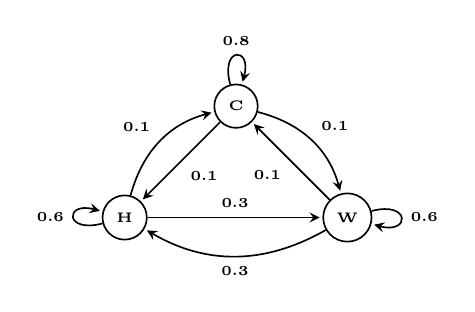
\begin{tikzpicture}[
				> = stealth, % arrow head style
				shorten > = 1pt, % don't touch arrow head to node
				auto,
				node distance = 2cm, % distance between nodes
				semithick, % line style
				font=\tiny\bfseries
				]
				
				\node[circle,draw] (qC) {C};
				\node[circle,draw] (qH) [below left of=qC] {H};
				\node[circle,draw] (qW) [below right of=qC] {W};
				
				\path[->] 	
				(qC) 	edge [loop above] node {0.8} ()
				edge [] node {0.1} (qH)
				edge [bend left] node {0.1} (qW)
				(qH) 	edge [loop left] node {0.6} ()
				edge [bend left] node {0.1} (qC)
				edge [] node {0.3} (qW)
				(qW)	edge [loop right] node {0.6} ()
				edge [bend left] node {0.3} (qH)
				edge [] node {0.1} (qC);
			\end{tikzpicture}
		\end{minipage}
		
		\begin{itemize}
			\item $\pi = [\pi_1, \pi_2, \ldots, \pi_n ]$: states initial probability distribution.
			\item $\sum_i \pi_i = 1$.
			\item E.g. \expword{Calculate the probability $P(H\, W\, C\, C)$ where $\pi = [0.1, 0.7, 0.2]$}.
		\end{itemize}
	\end{frame}
	
	\begin{frame}
		\frametitle{ML for NLP: \insertsection}
		\framesubtitle{\insertsubsection: Hidden Markov model}
		\begin{minipage}{.54\textwidth}
			\begin{itemize}
				\item $Q = \{q_1, q_2, \ldots, q_n\}$: states.
				\item $A$: transition probability matrix where $\sum_j a_{ij} = 1,\, \forall i$.
				\item $O = o_1 o_2 \ldots o_T$: sequence of observed events (words).
				\item $B = b_i(o_t)$: observation probabilities (\keyword{emission probabilities}), each represents the probability of generating an observation $o_t$ in a state $q_i$.
			\end{itemize}
		\end{minipage}
		\begin{minipage}{.45\textwidth}
			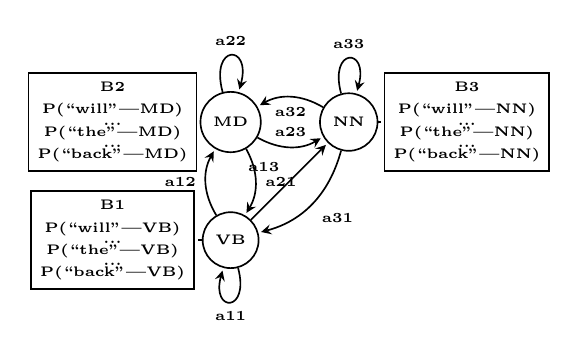
\begin{tikzpicture}[
				> = stealth, % arrow head style
				shorten > = 1pt, % don't touch arrow head to node
				auto,
				node distance = 1.5cm, % distance between nodes
				semithick, % line style
				font=\bfseries\fontsize{4}{4}\selectfont
				]
				
				\node[circle,draw] (q2) {MD};
				\node[align=center,draw] (q2e) [left of=q2] {B2\\ \\P(``will"|MD)\\...\\P(``the"|MD)\\...\\P(``back"|MD)};
				\node[circle,draw] (q3) [right of=q2] {NN};
				\node[align=center,draw] (q3e) [right of=q3] {B3\\ \\P(``will"|NN)\\...\\P(``the"|NN)\\...\\P(``back"|NN)};
				\node[circle,draw] (q1) [below of=q2] {VB};
				\node[align=center,draw] (q1e) [left of=q1] {B1\\ \\P(``will"|VB)\\...\\P(``the"|VB)\\...\\P(``back"|VB)};
				
				\path[->] 	
				(q1) 	edge [loop below] node {a11} ()
				edge [bend left] node {a12} (q2)
				edge [] node {a13} (q3)
				(q2) 	edge [loop above] node {a22} ()
				edge [bend left] node {a21} (q1)
				edge [bend right] node {a23} (q3)
				(q3)	edge [loop above] node {a33} ()
				edge [bend left] node {a31} (q1)
				edge [bend right] node {a32} (q2);
				
				\path[dashed] 	
				(q1) 	edge [] node {} (q1e)
				(q2) 	edge [] node {} (q2e)
				(q3) 	edge [] node {} (q3e);
				
			\end{tikzpicture}
		\end{minipage}
		
		\begin{itemize}
			\item $\pi = [\pi_1, \pi_2, \ldots, \pi_n ]$: states initial probability distribution.
			\item $\sum_i \pi_i = 1$.
		\end{itemize}
		
	\end{frame}
	
	\begin{frame}
		\frametitle{ML for NLP: \insertsection}
		\framesubtitle{\insertsubsection: Training}
		
		\begin{itemize}
			\item States are tags (categories) $t_i$.
			\item Let's define \keyword{START} as sentences start tag.
			\item The observations $o_i$ are the words $w_i$.
			\item \keyword{C}: Number of occurrences in the training corpus.
		\end{itemize}
		
		\begin{block}{HMM training}
			\[
			\text{Transition probabilities: } P(t_i | t_{i-1}) = \frac{C(t_{i-1}, t_i)}{C(t_{i-1})} 
			\]\[
			\text{Emission probabilities: } P(w_i | t_i) = \frac{C(t_i, w_i)}{C(t_i)}
			\]\[
			\text{Initial distribution: } \pi_i = P(t_i | START) = \frac{C(START, t_i)}{C(START)}
			\]
		\end{block}
	\end{frame}
	
	\begin{frame}
		\frametitle{ML for NLP: \insertsection}
		\framesubtitle{\insertsubsection: Labeling (tag decoding)}
		
		\begin{itemize}
			\item Given
			\begin{itemize}
				\item a Markov model $\lambda = (A, B)$,
				\item an observations (mots) sequence: $w = w_1 w_2 \ldots w_n$
			\end{itemize}
			\item Estimate a labels sequence $\hat{t} = \hat{t}_1 \hat{t}_2 \ldots \hat{t}_n$
		\end{itemize}
		
		\begin{block}{Labels decoding using HMM}
			\[
			\hat{t} = \arg\max\limits_t P(t | w) = \arg\max\limits_t \frac{P(w|t) P(t)}{P(w)} = \arg\max\limits_t P(w|t) P(t)%\text{ tel que } t = t_1 t_2 \ldots t_n
			\]
			
			\[ 
			P(w | t) \approx \prod\limits_{i=1}^n P(w_i|t_i) 
			\hskip2cm
			P(t) \approx \prod\limits_{i=1}^n P(t_i|t_{i-1}) 
			\]
			
			\[
			\hat{t} = \arg\max\limits_t \prod\limits_{i=1}^n P(w_i|t_i) P(t_i|t_{i-1})
			\]
		\end{block}
	\end{frame}
	
	\begin{frame}
		\frametitle{ML for NLP: \insertsection}
		\framesubtitle{\insertsubsection: Viterbi algorithm}
		
		\begin{block}{Viterbi}
			\scriptsize
			\begin{algorithm}[H]
%				\vskip-1em
				\KwData{$w = w_1 \ldots w_T$, HMM $\lambda = (A, B)$ with $N$ states}
				\KwResult{$best\_path$, $prob\_path$}
				
				Create a matrix $viterbi[N, T]$\;
				
				\lForEach{state $ s = 1 \ldots N$}{
					$viterbi[s, 1] = \pi_s * b_s(w_1);\, backpointer[s, 1] = 0$
				}
				
				\ForEach{tag $ t = 2 \ldots T$}{
					\ForEach{state $ s = 1 \ldots N$}{
						$viterbi[s, t] = \max\limits_{s'=1}^N viterbi[s', t-1] * a_{s',s} * b_s(w_t)$\;
						$backpointer[s, t] = \arg\max\limits_{s'=1}^N viterbi[s', t-1] * a_{s',s} * b_s(w_t)$\;
					}
				}
				
				$prob\_path = \max\limits_{s=1}^N viterbi[s, T];\, pointer\_path = \arg\max\limits_{s=1}^N viterbi[s, T]$\;
				
				$best\_path$ is the path starting from $pointer\_path$ and following $backpointer$
				
				\Return $best\_path$, $prob\_path$\;
				
			\end{algorithm}
		\end{block}
		
	\end{frame}
	
	\subsection{MEMM}
	
	\begin{frame}
		\frametitle{ML for NLP: \insertsection}
		\framesubtitle{\insertsubsection}
		
		\begin{itemize}
			\item Let's $x_{n}^{m} = x_n x_{n+1} \ldots x_{m-1} x_m$
			\item Given 
			\begin{itemize}
				\item an observations sequence (words): $w = w_1 w_2 \ldots w_n$
				\item a set of features $f$ defined on the sequences (such as: majuscule word)
			\end{itemize}
			\item Estimate tags sequence $\hat{t} = \hat{t}_1 \hat{t}_2 \ldots \hat{t}_n$
		\end{itemize}
		
		\begin{block}{Labels decoding using MEMM}
			\[
			\hat{t} = \arg\max\limits_t P(t | w) = \arg\max\limits_t \prod\limits_{i}  P(t_i | w_i, t_{i-1})
			\]
			
			\[
			\hat{t} = \arg\max\limits_t \prod\limits_{i}  
			\frac{exp\left(\sum_j \theta_j f_j(t_i, w_{i-l}^{i+l}, t_{i-k}^{i-1})\right)}%
			{\sum_{t' \in tags} exp\left(\sum_j \theta_j f_j(t'_i, w_{i-l}^{i+l}, t_{i-k}^{i-1})\right)}
			\]
		\end{block}
		
	\end{frame}
	
	\subsection{RNN}
	
	\begin{frame}
		\frametitle{ML for NLP: \insertsection}
		\framesubtitle{\insertsubsection: Examples}
		
		\vgraphpage{seq_class_RNN_exp.pdf}
		
	\end{frame}
	%===================================================================================
	\section{Attention}
	%===================================================================================
	
	\begin{frame}
		\frametitle{ML for NLP}
		\framesubtitle{\insertsection}
		
		\begin{itemize}
			\item Attention mechanism is used to give more importance to some part of the input data more than others.
			\item It improves capturing long-term information.
		\end{itemize}
		
	\end{frame}
	
	\subsection{Seq2Seq}
	
	\begin{frame}
		\frametitle{ML for NLP: \insertsection}
		\framesubtitle{\insertsubsection}
		
		\hgraphpage{seq2seq_exp.pdf}
		
	\end{frame}
	
	\subsection{Seq2Seq with attention}
	
	\begin{frame}
		\frametitle{ML for NLP: \insertsection}
		\framesubtitle{\insertsubsection}
		
		\vskip-3pt\hgraphpage{seq2seq_attention.pdf}
		
	\end{frame}
	
	\subsection{Attention types}
	
	\begin{frame}
		\frametitle{ML for NLP: \insertsection}
		\framesubtitle{\insertsubsection}
		
			\[Q \in \mathbb{R}^{n \times d}, \, K \in \mathbb{R}^{m \times d}, \, a(Q, K) \in \mathbb{R}^{n \times m}, V \in \mathbb{R}^{m \times v} \]
		
		\begin{itemize}
	
		\item Dot product (\textbf{tf.keras.layers.Attention})
		
		$ a(Q, K) = Q \cdot K^\top $
		
		\item Scaled dot product 
		
		$a(Q, K) = \frac{Q \cdot K^\top}{\sqrt{d}}$
		
		\item Cosine similarity
		
		$ a(Q, K) = \frac{Q \cdot K^\top}{||Q|| \, ||K||} $
		
		\item Additive attention (\textbf{tf.keras.layers.AdditiveAttention})
		
		Bahdanau Attention
		
		$ a(Q, K) = W_v^\top \cdot \tanh(W_q Q + W_k K) $
	\end{itemize}
		
	\end{frame}
	
	
	\subsection{Transformers}
	
	\begin{frame}
		\frametitle{ML for NLP: \insertsection}
		\framesubtitle{\insertsubsection: Multi-Head Attention}
		
		\vspace{-6pt}
		\begin{figure}
			\centering
			\hgraphpage[0.9\textwidth]{multi_head_att_.pdf}
			\vspace{-6pt}
			\caption{Multi-Head Attention \cite{2017-vaswani-al}}
		\end{figure}
	
	\end{frame}

	\begin{frame}
		\frametitle{ML for NLP: \insertsection}
		\framesubtitle{\insertsubsection: Multi-Head Attention}
		\begin{itemize}
			\item Q, K et V are trained using an MLP for each one
		\end{itemize}
		\[Q \in \mathbb{R}^{n \times d}, \, K \in \mathbb{R}^{m \times d}, \, MultiHead \in \mathbb{R}^{n \times d_{model}}, V \in \mathbb{R}^{m \times v} \]
		
		\[W^Q_i \in \mathbb{R}^{d_{model} \times d}, \,  W^K_i \in \mathbb{R}^{d_{model} \times d}, \, W^V_i \in \mathbb{R}^{d_{model} \times v}, \, W^O \in \mathbb{R}^{hv \times d_{model}}\]
		
		
		\[MultiHead(Q, K, V) = Concat(head_1, \ldots, head_h) \cdot W^O\]
		
		\[head_i = Attention(Q W^Q_i, K W^Q_i, V W^V_i)\]
	\end{frame}


	\begin{frame}
		\frametitle{ML for NLP: \insertsection}
		\framesubtitle{\insertsubsection: Multi-Head Attention}
		\vspace{-6pt}
		\begin{figure}
			\centering
			\hgraphpage[0.35\textwidth]{transformers_.pdf}
			\vspace{-6pt}
			\caption{Transformers architecture \cite{2017-vaswani-al}}
		\end{figure}
	\end{frame}

	
	\insertbibliography{NLP02}{*}
	
\end{document}

